\chapter{Theoretical overview}
\label{chap:Theory}

\chapterquote{I believe it is impossible to be sure of anything.}%
{Han Fei Zi, 280 BC $-$ 233 BC}%: Blackwood's Magazine May 1830

This chapter provides a review of the Standard Model of Particle Physics, with an emphasis on the Higgs mechanism and the Higgs boson.  A general parametrisation of the Higgs theory is discussed, which supplies the theoretical background for the physics analysis in \Chapter{chap:DoubleHiggs}. Lastly a discussion of the usage of  the tau pair polarisation correlations as a signature of Higgs boson is presented, which motivates the study in \Chapter{chap:Tau2Mini}.


\section{Overview of the Standard Model}

The Standard Model (\SM) \cite{Agashe:2014kda,Thomson:2013zua,Tong:QFT,Gripaios:GFT} is a quantum field theory concerning the fundamental particles and three fundamental interactions of nature: the electromagnetic; the weak; and the strong interactions.  The fundamental particles in the \SM consist of bosons and fermions. The bosons mediate the fundamental forces between particles: the photon is the force carrier of the electromagnetic force; \PWp, \PWm, and \PZ  bosons are the force carriers of the weak force; and the gluon, \Pg, is the force carrier of the strong force. The properties of the force-exchange bosons and Higgs boson are listed in \Table{tab:theoryBoson}.


\begin{table}[htbp]
\centering
\smallskip
\begin{tabular}{l  r r rr }
\hline
\hline
Force &  Boson & Mass & Spin & Charge / $e$ \\
\hline
Electromagnetic & photon & 0 & 1 & 0 \\
\hline
\multirow{3}{*}{Weak}   & \PWplus & 80.385(15)\,GeV & 1 & 1 \\
  & \PWminus & 80.385(15)\,GeV & 1 &  $-1$ \\
  & \PZ & 91.1876(21)\,GeV & 1 &  0 \\
\hline
Strong  & gluon & 0 & 1 & 0 \\
\hline
 - & Higgs & 125.1(3)\,GeV & 0 & 0 \\
\hline
\hline
\end{tabular}

\caption
{Masses, spins, and charges of fundamental bosons in the \SM. Values are taken from \cite{Agashe:2014kda}.}
\label{tab:theoryBoson}
\end{table}





The other  fundamental particles are spin-$\frac{1}{2}$ fermions. For each fermion in the \SM, there is an anti-fermion with the same mass and spin, but opposite charge. These fermions  have three generations. Each generation of fermions has the same interaction property, but different masses. Experimental evidences of three generations include the measurements of the \PZ boson decay-width, which strongly suggested three generations of neutrinos \cite{ALEPH:2005ab}.

These fermions come in two distinct categories: leptons and quarks.  Neutral leptons (the neutrinos) only experience the weak forces. Charged leptons (\Pepm, \Pmupm, \Ptaupm) experience the weak forces and the electromagnetic forces. Quarks experience all three fundamental forces described by the \SM. Properties of these fermions are listed in \Table{tab:theoryFermion}.


\begin{table}[htbp]
\centering
\smallskip
\begin{tabular}{l  r r r r }
\hline
\hline
Type&Generation &  Fermion & Mass & Charge / $e$ \\
\hline
\multirow{6}{*}{Lepton} & \multirow{2}{*}{1}  & \Pem & 0.548579909070(16)\,MeV & $-1$ \\
 &   & \Pnue & - & 0 \\\cline{2-5}
 & \multirow{2}{*}{2}  & \Pmuon & 105.6583745(24)\,MeV & $-1$ \\
 &   & \Pnum & - & 0 \\\cline{2-5}
 & \multirow{2}{*}{3}  & \Ptauon & 1776.86(12)\,MeV & $-1$ \\
 &   & \Pnut & - & 0 \\
\hline
\multirow{6}{*}{Quark} & \multirow{2}{*}{1}  & \Pup & $2.2^{+0.6}_{-0.4}$\,MeV & $+\frac{2}{3}$ \\
 &   & \Pdown & $4.7^{+0.5}_{-0.4}$\,MeV & $-\frac{1}{2}$ \\\cline{2-5}
 & \multirow{2}{*}{2}  & \Pcharm & 1270$\pm$30\,MeV & $+\frac{2}{3}$ \\
 &   & \Pstrange & $98^{+8}_{-4}$\,MeV & $-\frac{1}{3}$ \\\cline{2-5}
 & \multirow{2}{*}{3}  & \Ptop & 173210$\pm510\pm710$\,MeV & $+\frac{2}{3}$ \\
 &   & \Pbottom & $4180^{+40}_{-30}$\,MeV & $-\frac{1}{3}$ \\
\hline
\hline
\end{tabular}

\caption
{Masses and charges of the fundamental fermions in the \SM. All fermions are spin-$\frac{1}{2}$ particles. For each fermion in the \SM, there is an anti-fermion with the same mass and spin, but opposite charge. Neutrinos are known to have non-zero masses from the observation of neutrino flavour oscillations. The upper bound on the neutrino mass is 2\,eV. For the top quark mass, the statistical uncertainty is listed first, followed by the systematic uncertaintiy. Values are taken from \cite{Agashe:2014kda}.}
\label{tab:theoryFermion}
\end{table}

\begin{comment}


In theoretical physics, quantum field theory (QFT) is the theoretical framework for constructing quantum mechanical models of subatomic particles in particle physics and quasiparticles in condensed matter physics. QFT treats particles as excited states of the underlying physical field, so these are called field quanta.

In quantum field theory, quantum mechanical interactions among particles are described by interaction terms among the corresponding underlying quantum fields. These interactions are conveniently visualized by Feynman diagrams, which are a formal tool of relativistically covariant perturbation theory, serving to evaluate particle processes.

In physics, a gauge theory is a type of field theory in which the Lagrangian is invariant under a continuous group of local transformations. An invariant is a model that holds true no matter the mathematical procedure applied to it. This is the concept behind gauge invariance. The idea of fields as described by Michael Faraday in his study of electromagnetism led to the postulate that fields could be described mathematically as scalars and vectors. When a field is transformed, but the result is not, this is called gauge invariance or gauge symmetry.[1] Applying gauge theory creates a unification which describes mathematical formulas or models that hold well for all fields of the same class.



The \SM also describes the interactions between sub-atomic particles. The deployment and the experimental verification of the \SM throughout the second half of the 20th century is one of the greatest triumphs of particle physics. The recent discovery of the Higgs boson in 2012 \cite{Aad:2012tfa,Chatrchyan:2012ufa} further verified the theory. This chapter summarises the \SM based on the reviews of the \SM presented in \cite{Agashe:2014kda,Thomson:2013zua,Tong:QFT,Gripaios:GFT}.



%A summary of the selected properties of these force exchange bosons can be found in \Table{}.

Another category of fundamental particles contains leptons and neutrinos. These particles are fermions. For each fermion in the \SM, there is an anti-fermion with the same mass and spin, but opposite charge. Leptons and neutrinos have three generations. Each generation has the same interaction properties, but different masses. Although neutrinos could not be directly detected, measurements of the \PZ decay-width strongly suggested three generations of neutrinos \cite{ALEPH:2005ab}. Leptons and neutrinos experience weak forces as well as electromagnetic forces.

\end{comment}

Many \SM predications have been experimentally verified. Some recent highlights include the discovery of the top quark in 1995 \cite{Abachi:1995iq}, the tau neutrino in 2000 \cite{Kodama:2000mp}, and the Higgs boson in 2012 \cite{Aad:2012tfa,Chatrchyan:2012ufa}. However, there are observations which are not explained by the \SM. One issue is that the \SM does not incorporate the gravitational force. Another issue is that the \SM does not natively allow neutrino masses and mixings. The \SM also does not explain the existence of the dark matter. There are many theories beyond the Standard Model (BSM) trying to provide an explanation for these issues. One example is the generalisation of the Higgs theory to allow non-SM coupling strengths \cite{Kaplan:1983fs,Goldberger:2008zz}.

%The overview of the Standard Model starts with the quantum electrodynamics, and its generalisation to quantum chromodynamics. The unification of electromagnetism and the weak interaction, the electroweak gauge theory, will be discussed. Afterwards, the Higgs mechanism and Yukawa couplings will be introduced to explain masses of bosons and fermions whilst preserving the Lagrangian symmetry. This will be followed by a detailed discussion on the Standard Model Higgs boson, its mass and interactions with other particles. The chapter moves to an explanation of possible Higgs theories beyond the Standard Model, with their  Lagrangian of the Higgs interaction and observables. Lastly the discussion is provided on  the tau pair polarisation correlation as a signature for Higgs boson. This signature could be used to identify Higgs boson if an excess of tau pair decay events observed among all lepton pair decay events.

\begin{comment}
\section{Notations and conventions}

Natural unit is used in this thesis: $\hbar = c = 1$. The metric is mostly-minus, $\eta^{\mu\nu} = \text{diag}(1,-1,-1,-1)$. The Dirac gamma matrices are represented with $\gamma^{\mu}$, with $\mu\in\braces{0,1,2,3}$. $\gamma^5 = i \gamma^{0}\gamma^{1}\gamma^{2}\gamma^{3}$. $\overline{\psi} = \psi^{\dagger}\gamma^0$. Einstein summation convention is also used in this thesis.

This set of notations allow a contracted pair to be a Lorentz invariant. For a Weyl spinor, $\psi_\alpha$, the mass term in the Lagrangian is of the form $\psi^{\alpha}\psi_\alpha$, which is the Majorana mass term. The contracted pair between two different Weyl spinors would form a Dirac mass term.
\end{comment}

\section{Quantum electrodynamics}


 \QED is a  quantum gauge field theory explaining electromagnetic interactions. Quantum field theory (QFT) is the theoretical framework for constructing quantum mechanical models of fundamental particles. Particles are treated as excited states of the underlying physical field in the QFT.  A gauge theory is a type of field theory in which the Lagrangian is invariant under a continuous group of local transformations.  Gauge invariance or gauge symmetry refers to when a field is transformed, but the Lagrangian is not.

\QED is an abelian gauge theory with the  U(1) symmetry group. The gauge field, which mediates the interaction between the charged spin-$\frac{1}{2}$ fields, is the electromagnetic field, denoted $A^{\mu}$. The \QED Lagrangian \cite{peskin1995introduction} for a spin-$\frac{1}{2}$ field interacting with the electromagnetic field is given by:
\begin{equation}
\Lagr_{QED} = \overline{\psi} \left( i\Dstroke - m \right)\psi -  \frac{1}{4}F_{\mu\nu}F^{\mu\nu},
\end{equation}
where $\psi$ is the spin-$\frac{1}{2}$ Dirac field satisfying the Dirac equation, given by the Lagrangian density:
\begin{equation}
\Lagr =  \overline{\psi} \left( i\Dstroke - m \right)\psi,
\end{equation}
where the $\gamma^{\mu}$ are the Dirac gamma matrices with $\mu\in\braces{0,1,2,3}$; $\overline{\psi}$ is defined as $\psi^{\dagger}\gamma^0$; $F_{\mu\nu} = \partial_{\mu}A_{\nu} - \partial_{\nu}A_{\mu}$ is the electromagnetic field tensor; $e$ is the coupling constant, which is equal to the electric charge; $m$ is the mass of the electron; and the gauge covariant derivative is given by:
\begin{equation}
D_{\mu} \equiv \partial_{\mu} + ieA_{\mu},
\end{equation}
where $A_{\mu}$ is the covariant four-vector potential of the electromagnetic field generated by the electron itself.


\begin{comment}

\QED describes the interaction between a spin-$\frac{1}{2}$ Dirac field, $\psi$, and a vector field, $A_{\mu}$. The Dirac field, $\psi$, satisfies the Dirac equation, given by the Lagrangian density:
\begin{equation}
\Lagr =  \overline{\psi} \left( i\Dstroke - m \right)\psi,
\end{equation}
where


QED is an abelian gauge theory with the symmetry group U(1). The gauge field, which mediates the interaction between the charged spin-1/2 fields, is the electromagnetic field.


The natural starting point to introduce the \SM is with quantum electrodynamics (\QED). The \QED is a quantum field theory explaining electromagnetic interactions. The theory involves a spin-half Dirac (electron) field, $\psi$, and a vector (photon) field, $A_{\mu}$. When the local (gauge) symmetry is imposed, which is equivalent to the Lagrangian invariance under transformations,
\begin{equation}
\psi\ \to\ e^{i\phi(x)}\psi,\ A_{\mu}\ \to\ A_{\mu} - \partial^{\mu}\phi(x),
\end{equation}
the Lagrangian is fixed to be:
\begin{equation}
\Lagr_{QED} = \overline{\psi} \left( i\Dstroke - m \right)\psi -  \frac{1}{4}F_{\mu\nu}F^{\mu\nu},
\end{equation}
if up to cubic terms are allowed in the fields. Here $D_{\mu} = \partial_{\mu} + ieA_{\mu}$ and $F_{\mu\nu} = \partial_{\mu}A_{\nu} - \partial_{\nu}A_{\mu}$. There are two free parameters in \QED: $m$, the electron mass, and $e$, the electron charge. The mass term for the photon, $\nu^{2}A_{nu}A^{\nu}$, is forbidden by gauge invariance.

\QED has been verified experimentally. One of its greatest prediction is the spin magnetic dipole moment of the electron, $g_{s}$, which is predicted to be  2 from the Dirac equations, plus small corrections to the value that comes from the electron's interaction with virtual photons, so called higher ``loop'' corrections in Feynman diagrams. The current best calculated \QED prediction states $g=2.001159652181643(764)$ \cite{Aoyama:2014sxa}, where the best experimental value and uncertainty is $g = 2.00115965218073(28)$ \cite{Hanneke:2010au}. Precise agreement of the theoretical prediction and the experimental value, 1 part in \text{$10^{12}$}, is a success of the \QED.
\end{comment}
% , defined as $\vec{\mu} = g_{s}\frac{Qq}{2m} \vec{s}$
\begin{comment}
The Standard Model of particle physics is a theory concerning the electromagnetic, weak, and strong interactions, as well as classifying all the elementary particles known. It was developed throughout the latter half of the 20th century, as a collaborative effort of scientists around the world.[1] The current formulation was finalized in the mid-1970s upon experimental confirmation of the existence of quarks. Since then, discoveries of the top quark (1995), the tau neutrino (2000), and the Higgs boson (2012) have given further credence to the Standard Model. Because of its success in explaining a wide variety of experimental results, the Standard Model is sometimes regarded as the "theory of almost everything".

Although the Standard Model is believed to be theoretically self-consistent[2] and has demonstrated huge and continued successes in providing experimental predictions, it does leave some phenomena unexplained and it falls short of being a complete theory of fundamental interactions. It does not incorporate the full theory of gravitation[3] as described by general relativity, or account for the accelerating expansion of the Universe (as possibly described by dark energy). The model does not contain any viable dark matter particle that possesses all of the required properties deduced from observational cosmology. It also does not incorporate neutrino oscillations (and their non-zero masses).

The development of the Standard Model was driven by theoretical and experimental particle physicists alike. For theorists, the Standard Model is a paradigm of a quantum field theory, which exhibits a wide range of physics including spontaneous symmetry breaking, anomalies and non-perturbative behavior. It is used as a basis for building more exotic models that incorporate hypothetical particles, extra dimensions, and elaborate symmetries (such as supersymmetry) in an attempt to explain experimental results at variance with the Standard Model, such as the existence of dark matter and neutrino oscillations.
\end{comment}

\section{Quantum chromodynamics}

Quantum chromodynamics (\QCD) is the quantum field theory of strong interactions. \QCD theory is invariant under local non-Abelian SU(3) transformations. There are eight gauge bosons, the gluons, corresponding to the eight ($8 = 3^2 - 1$) generators of the SU(3) symmetry group. Gluons carry colour charges. There are three types of colour charges, sometimes labelled as red, green, and blue. Anti-particles carry anticolour. Quarks are associated with a single colour. Gluons are made up of a colour and an anticolour (or superposition of colour$-$anticolour pair). The \QCD Lagrangian is given by:
\begin{equation}
\Lagr_{QCD} = \sum_{f\in{u,d,s,c,b,t}} \overline{\psi_i} \left(\parenths{ i\gamma^{\mu}\partial_{\mu} - g_{s}\gamma^{\mu}G^a_{\mu}\frac{\lambda^a}{2}}_{ij} - m_f\delta_{ij} \right)\psi_j -  \frac{1}{4}G^a_{\mu\nu}G^{a\mu\nu},
\end{equation}
where $\psi$ represents a quark  with a colour charge, indicated by $i$ or $j$; $m$ controls the mass of the quark; $g_s$ is the strong coupling constant; $a$ is the colour charge; $\lambda^a$ represents one of the eight Gell-Mann matrices; and $G^a_{\mu\nu}$ represents the gauge invariant gluon field strength tensor, given by:
\begin{equation}
G^a_{\mu\nu} = \partial_{\mu}\gamma_{\nu}^a - \partial_{\nu}\gamma_{\mu}^a  - g_{s}f_{abc}G_{\mu}^{b}G_{\nu}^c,
\end{equation}
where $G_{\mu}^{b}$ is the gluon field with colour charge $b$.

\section{The electroweak interaction}
\label{sec:theoryElectroweak}

The electroweak interaction can be thought as an extension to \QED to incorporate the weak force, the force describing nuclear radioactive decay. The unification of the electromagnetic and the weak force is accomplished under an \uprightMath{SU(2)_L \times U(1)} gauge symmetry group. The corresponding gauge bosons are  three \PW bosons ($W^1$, $W^2$, and $W^3$) from \uprightMath{SU(2)_L} gauge symmetry, and  $B$ boson from U(1) gauge symmetry. All gauge bosons are initially massless. Fermion mass terms are forbidden under  \uprightMath{SU(2)_L} gauge symmetry.

The electroweak Lagrangian can be written as
\begin{equation}
\Lagr_{Electroweak} = \Lagr_{Boson} + \Lagr_{Fermion} + \Lagr_{Higgs} + \Lagr_{Yukawa}.
\end{equation}

First consider $\Lagr_{Boson}$, given by:
\begin{equation}
\Lagr_{Boson} = - \frac{1}{4} W^i_{\mu\nu} W^{i\mu\nu} - \frac{1}{4}B_{\mu\nu} B^{\mu\nu},
\label{eq:theoryEWBoson}
\end{equation}
\begin{equation}
W^i_{\mu\nu} = \partial_{\nu}W^i_{\mu} - \partial_{\mu}W^i_{\nu} - g\varepsilon^{ijk}W^j_{\mu}W^k_\nu ,
\end{equation}
\begin{equation}
B_{\mu\nu} = \partial_{\nu}B_{\mu} - \partial_{\mu}B_{\nu},
\end{equation}
where $B$ field  is invariant under U(1) transformations; $W$ field is invariant under non-Abelian SU(2) transformations; and the indices, $i$, $j$, and $k$, indicate three $W$ fields.


The term $\Lagr_{Fermion}$ describes the massless fermion fields coupling to the fermions, and the propagation of the fermion fields. The left-handed ($ \psi_L $) and the right-handed fermions ($ \psi_R $) are treated differently. The right-handed fermions are singlets. The left-handed fermions are in doublets with the corresponding fermions of the same generation. The term $\Lagr_{Fermion}$ is given by:
\begin{equation}
\Lagr_{Fermion} = \sum_{\psi\in{fermions}} {\overline{\psi}}_L \gamma^{\mu}D^L_{\mu} \psi_L +  \overline{\psi}_R \gamma^{\mu}D^R_{\mu} \psi_R ,
\end{equation}
where covariant derivatives $D^L_{\mu}$ and $D^R_{\mu}$ are defined as
\begin{equation}
D^L_{\mu} & = \partial_{\mu} + ig\frac{\tau_i}{2}W^i_{\mu} + ig'Y_{\psi}B_{\mu} , \\
D^R_{\mu} & = \partial_{\mu}  + ig'Y_{\psi}B_{\mu} .
\end{equation}
The structure of this Lagrangian allows $W$ and $B$ fields to couple with left-handed fermions, but only allows the $B$ field to couple with right-handed fermions. The $\tau_i$ matrices are the generators of SU(2) and $Y_{\psi}$ is the hypercharge associated with the fermion field $\psi$. The $W$ field couples with strength $g$ to the fermion field. The $B$ field couples with strength $g'$ to the particles carrying weak hypercharge $Y$.

%The four vector fields ($W^1$, $W^2$, and $W^3$, $B$) are massless.
The term $\Lagr_{Higgs}$ describes the Higgs field. After electroweak symmetry breaking of the Higgs field, the mass terms of the gauge bosons are introduced. The term $ \Lagr_{Yukawa}$ produces the mass terms of the quarks and charged leptons. Firstly a general  spontaneous symmetry breaking mechanism is provided, followed by a description of the electroweak symmetry breaking.

%The mass of the physical bosons and fermions are obtained via electroweak symmetry breaking.

\subsection{Spontaneous symmetry breaking}

Consider a complex scalar field, with the Klein-Gordon Lagrangian:
\begin{equation}
\Lagr = \partial^\mu{\psi}^*\partial_\mu\psi - m^2 \absOf{\psi}^2 =  \partial^\mu{\psi}^*\partial_\mu\psi - V\parenths{\psi} ,
\label{eq:theoryKGLagrangian}
\end{equation}
where $m$ is the mass term and $V\parenths{\psi} $ is the potential of the field $\psi$. This Lagrangian has a global symmetry $\psi \to e^{i\phi}\psi$. The potential can be modified to add an interaction term without breaking the  invariance of the global symmetry:
\begin{equation}
V\parenths{\psi} =  m^2 \absOf{\psi}^2 + \lambda\absOf{\psi}^4,
\end{equation}
where $\lambda$ controls the interaction strength. This modified potential has a minimum at $ \absOf{\psi}=0$ for $m^2>0$. However, if $m^2<0$, the minimum of the potential occurs when:
\begin{equation}
\frac{\partial{V}\parenths{\psi}}{\partial{\absOf{\psi}}} =  2 m^2 \absOf{\psi} + 4\lambda\absOf{\psi}^3 = 0,
\end{equation}
leading to a non-negative expectation value for the field:
\begin{equation}
\absOf{\psi} = \sqrt{\frac{-m^2}{2\lambda}}\equiv \frac{\nu}{\sqrt{2}},
\end{equation}
where $\nu = \sqrt{-m^2/\lambda}$. The solution that minimises the potential is not unique; it corresponds to a circle of points in the complex $\psi$ plane. By choosing any one of these points, which are degenerate in energy, the symmetry of   $\psi \to e^{i\phi}\psi$ is broken. This phenomenon is known as the spontaneous symmetry breaking.

A consequence of  spontaneous symmetry breaking is that the perturbation of the field along the degenerate energy direction, which is the circle in complex $\psi$ plane, have no associated potential energy. This is formalised as Goldstone's theorem \cite{Nambu:1960tm,Goldstone:1961eq}. The theorem states that spontaneous symmetry breaking always implies the existence of a massless particle.

To demonstrate Goldstone's theorem, using the Lagrangian in \Equation{eq:theoryKGLagrangian} as an example, after the spontaneous symmetry breaking of the field, the perturbation of the field $\psi$ near the field minimum point can be written as
 \begin{equation}
\psi = \frac{1}{\sqrt{2}}\parenths{\nu+\psi_1+i\psi_2},
\end{equation}
where $\nu=\sqrt{{-m^2}/{\lambda}}$ refers to the minimum point in the potential, and $\psi_1$ and $\psi_2$ are real scalar fields. Substituting $\psi$ in the Lagrangian in \Equation{eq:theoryKGLagrangian} gives:
\begin{equation}
\Lagr = \frac{1}{2}\partial^\mu{\psi_1}\partial_\mu\psi_1 + \frac{1}{2}\partial^\mu{\psi_2}\partial_\mu\psi_2 - m^2 \psi_1^2 + \hdots.
\end{equation}
The mass term for the $\psi_1$ field is $\sqrt{-m^2}$ whereas there is no mass term for the $\psi_2$ field, as stated by the Goldstone's theorem.

In the previous example, the Lagrangian in \Equation{eq:theoryKGLagrangian} possesses  the global symmetry of $\psi \to e^{i\phi}\psi$. Instead, if there is a local U(1) gauge symmetry of  $\psi \to e^{i\phi(x)}\psi$, this implies a corresponding field $A_{\mu}$, which transforms as $A_\mu \to A_\mu - \partial_\mu\phi(x)$. For the gauge invariance, the covariant derivative becomes $D_\mu = \partial_\mu+ieA_\mu$. Hence the Lagrangian in \Equation{eq:theoryKGLagrangian} becomes:
\begin{equation}
\Lagr = \parenths{D^\mu{\psi}}^*\parenths{D_\mu\psi} - m^2 \absOf{\psi}^2    - \lambda\absOf{\psi}^4.
\end{equation}
When the field is expanded around the minimum of the potential,  $\nu=\sqrt{{-m^2}/{\lambda}}$, with $m^2<0$,  the gauge boson mass term
\begin{equation}
+\frac{e^2\nu^2}{2}A^\mu{A}_\mu,
\end{equation}
 is obtained from the $\parenths{D^\mu{\psi}}^*\parenths{D_\mu\psi} $ term in the Lagrangian. Therefore the spontaneous symmetry breaking of a gauge field gives rise to a gauge boson mass.

\section{Higgs Mechanism}
\label{sec:theoryHiggs}

The Higgs mechanism is an extension of the example of the spontaneous symmetry breaking introduced in the previous section. It can provide mass terms for bosons and fermions that are compatible with the gauge invariance of the \SM. A complex  scalar Higgs field, $\Phi_{\PH}$, transforms as a doublet of SU(2) with hypercharge $Y = \frac{1}{2}$. The Higgs Lagrangian is given by:
\begin{equation}
\Lagr_{Higgs} = \left(D_\mu\Phi_{\PH}\right)^\dagger\left(D^\mu\Phi_{\PH}\right) - \mu^2\Phi_{\PH}^\dagger\Phi_{\PH} + \lambda\left(\Phi_{\PH}^\dagger\Phi_{\PH}\right)^2,
\label{eq:theoryEWSBhiggs}
\end{equation}
where $\lambda$ and $\mu$ are constants. The \uprightMath{SU(2)_L\times U(1)} symmetry of the electroweak  Lagrangian demands that the covariant derivative of the  Higgs field takes the form
\begin{equation}
D_\mu = \left(\partial_{\mu} + ig\frac{\tau_i}{2}W^i_{\mu} + ig'\frac{1}{2}B_{\mu}\right),
\end{equation}
where $g$ is the coupling constant of the \uprightMath{SU(2)_L} gauge symmetry; $g'$ is the coupling constant of the U(1) gauge symmetry; and the $\tau_i$ are Pauli matrices. The Higgs potential is given by:
\begin{equation}
V(\PH) = \mu^2\Phi_{\PH}^\dagger\Phi_{\PH} - \lambda\left(\Phi_{\PH}^\dagger\Phi_{\PH}\right)^2.
\label{eq:theoryHiggsPotential}
\end{equation}
The Higgs potential is minimised when
\begin{equation}
\sqrt{\Phi_{\PH}^\dagger\Phi_{\PH}} =  \frac{\nu}{\sqrt{2}}=\sqrt{\frac{\mu^2}{2\lambda}}.
\end{equation}
By expanding the Higgs field about the minimum point of the potential, the non-zero vacuum expectation value (VEV) can be written as:
 \begin{equation}
\angles{\Phi_{\PH}} =
\begin{pmatrix}
0 \\
\frac{\nu}{\sqrt{2}}
\end{pmatrix}
,
\end{equation}
with a real $\nu$. Substituting the  Higgs VEV into the $\Lagr_{Higgs}$ in \Equation{eq:theoryEWSBhiggs}, the $\left(D_\mu\Phi_{\PH}\right)^\dagger\left(D^\mu\Phi_{\PH}\right)$ term becomes
 \begin{equation}
-\frac{1}{8}
\begin{pmatrix}
0 & \nu
\end{pmatrix}
\begin{pmatrix}
gW^3_\mu+g'B_\mu & g\parenths{W^1_\mu-iW^2_\mu} \\
g\parenths{W^1_\mu+iW^2_\mu} &  -gW^3_\mu+g'B_\mu
\end{pmatrix}
\begin{pmatrix}
gW^3_\mu+g'B_\mu & g\parenths{W^1_\mu-iW^2_\mu} \\
g\parenths{W^1_\mu+iW^2_\mu} &  -gW^3_\mu+g'B_\mu
\end{pmatrix}
\begin{pmatrix}
0 \\
\nu
\end{pmatrix}.
\label{eq:theoryEWBosonMass1}
\end{equation}
Ignoring the negative sign, the expression simplifies to
\begin{equation}
\frac{\nu^2g^2}{8}\parenths{W^1_\mu-iW^2_\mu}\parenths{W^1_\mu+iW^2_\mu} + \frac{\nu^2}{8}\parenths{gW^3_\mu - g'B_\mu}^2.
\label{eq:theoryGaugeBonson1}
\end{equation}
The physical fields $W^+_{\mu}$ and $W^-_{\mu}$ can be identified with the first part of the \Equation{eq:theoryGaugeBonson1}, as
\begin{equation}
W^+_{\mu} & = \frac{1}{\sqrt{2}}\parenths{W^1_\mu-iW^2\mu}, \\
W^-_{\mu} & = \frac{1}{\sqrt{2}}\parenths{W^1_\mu+iW^2\mu}.
\end{equation}
The physical fields $Z_{\mu}$ and $A_{\mu}$ are associated with $W^3_{\mu}$ and $B_{\mu}$. Since the \PZ boson is massive and the photon is massless, the second part of the \Equation{eq:theoryGaugeBonson1} should give rise to \PZ boson mass term only, with no mass term for photon. This can be achieved by rearranging the second part of the \Equation{eq:theoryGaugeBonson1}:
\begin{equation}
\frac{\nu^2}{8}\parenths{gW^3_\mu - g'B_\mu}^2 = \frac{\nu^2\parenths{g^2+{g'}^2}}{8}\parenths{\frac{g}{\sqrt{g^2+{g'}^2}}W^3_\mu - \frac{g'}{\sqrt{g^2+{g'}^2}}B_\mu}^2.
\label{eq:theoryEWBosonMass2}
\end{equation}
A convenient way to connect $g$ and $g'$ is to use the Weinberg mixing angle  \cite{Weinberg:1967tq}, denoted as \weinberg. The Weinberg mixing angle is defined as
\begin{equation}
\cos\parenths{\weinberg} & = \frac{g}{\sqrt{g^2+{g'}^2}},\\
\sin\parenths{\weinberg} & = \frac{g'}{\sqrt{g^2+{g'}^2}}.
\end{equation}
The \Equation{eq:theoryEWBosonMass2} can be rewritten using the Weinberg mixing angle:
\begin{equation}
\frac{\nu^2\parenths{g^2+{g'}^2}}{8}\parenths{\cos\parenths{\weinberg}W^3_\mu - \sin\parenths{\weinberg}B_\mu}^2.
\label{eq:theoryEWBosonMass3}
\end{equation}
The physical field $Z_{\mu}$ can be immediately identified as:
\begin{equation}
Z_{\mu} = \cos\parenths{\weinberg}W^3_{\mu} - \sin\parenths{\weinberg}B_{\mu}.
\end{equation}
Consequently, the physical field $A_{\mu}$ with associated massless photon can be written as:
\begin{equation}
A_{\mu} = \sin\parenths{\weinberg}W^3_{\mu} + \cos\parenths{\weinberg}B_{\mu}.
\end{equation}
The \Equation{eq:theoryGaugeBonson1} can be written in terms of the physical fields $W^+_{\mu}$, $W^-_{\mu}$, $Z_{\mu}$, and $A_{\mu}$:
\begin{equation}
\frac{{\left(g\nu\right)}^2}{4}W^+_{\mu}W^{-\mu} + \frac{\left(g^2 + {g'}^{2}\right)\nu^2}{8}Z_{\mu}Z^{\mu}.
\label{eq:theoryBoson}
\end{equation}
The first term gives mass of the \PWplus and \PWminus vector bosons. The second term gives mass of the \PZ vector boson. There is no mass term for the photon. The spontaneous symmetry breaking of the Higgs field breaks the electroweak  \uprightMath{SU(2)_L\times U(1)} gauge symmetry to the U(1)  gauge symmetry of the electromagnetism.  The masses of the \PWplus, \PWminus and \PZ bosons are given by:
\begin{equation}
m_{\PWplus} = m_{\PWminus} = \frac{g\nu}{2},\quad m_{\PZ} = \frac{\nu\sqrt{g^2+{g'}^2}}{2} = \frac{m_{\PW}}{\cos\parenths{\weinberg}}.
\end{equation}

\begin{comment}





Assuming there is a mixing of the $SU(2)_L$ and $U(1)$ fields:
\begin{equation}
Z_{\mu} = \cos\left(\theta_W\right)W^3_{\mu} - \sin\left(\theta_W\right)B_{\mu},
\end{equation}
\begin{equation}
A_{\mu} = \sin\left(\theta_W\right)W^3_{\mu} + \cos\left(\theta_W\right)B_{\mu},
\end{equation}
\begin{equation}
W^+_{\mu} = \frac{1}{2}\parenths{W^1_\mu-iW^2\mu},
\end{equation}
\begin{equation}
W^-_{\mu} = \frac{1}{2}\parenths{W^1_\mu+iW^2\mu},
\end{equation}
the gauge boson mass matrix in \Equation{eq:theoryEWBosonMass1} can be simplified to:
\begin{equation}
\frac{{\left(g\nu\right)}^2}{4}W^+_{\mu}W^{-\mu} + \frac{\left(g^2 + g^{'2}\right)\nu^2}{8}Z_{\mu}Z^{\mu}.
\label{eq:theoryBoson}
\end{equation}
Hence the gauge boson masses obtained from the spontaneous symmetry breaking of the Higgs fields are:
\begin{equation}
m_{\PWplus} = m_{\PWminus} = \frac{g\nu}{2},
\end{equation}
\begin{equation}
m_{\PZ} = \frac{\nu\sqrt{g^2+{g'}^2}}{2} = \frac{m_{\PW}}{\cos\parenths{\theta{\PW}}},
\end{equation}
\begin{equation}
m_{A} = 0,
\end{equation}
where $\theta_{\PW}$ is the Weinberg mixing angle \cite{Weinberg:1967tq}, which is determined experimentally. This produces  a massless gauge boson with the $A_\mu$ field, associated with the physical photon; two massive  gauge bosons with $W^+_{\mu}$ and $W^-_{\mu}$ field, associated with physical \PWplus and \PWminus bosons; and a massive boson with $Z_{\mu}$ field, associated with physical \PZ boson. Consequently, the spontaneous symmetry breaking of the Higgs field breaks the electroweak  $SU(2)_L\times U(1)$ symmetry to electromagnetism U(1) symmetry.
\end{comment}

\section{Higgs boson}
\label{sec:theoryHiggsBoson}

%So far, interactions between different fields in the Standard Model, as well as the boson and fermion masses obtaining mechanisms, have been discussed. The only thing left for discussion is the Higgs boson, and  interactions between the Higgs boson and other fields.

For the Higgs doublet complex field in the \SM, there are four real scalar degrees of freedom. Three degrees of freedom are ``eaten'' to form the longitudinal polarisations of the $W^{\pm}_\mu$ and $Z_\mu$ fields. The remaining one real scalar degree of freedom forms the Higgs boson. The properties of the Higgs bosons can be shown in the unitary gauge, where three degrees of freedom are manifestly eaten. The Higgs field is given by:
\begin{equation}
H(x) = \frac{1}{\sqrt{2}}
 \begin{pmatrix}
  0 \\
  \nu + h(x) \\
 \end{pmatrix},
\end{equation}
where $h(x)$ is the real scalar field of the Higgs boson and $\nu$ the Higgs vacuum expectation value. The Higgs boson is not charged under electromagnetism as the field is real. The coupling of the Higgs boson to other fields  can be calculated out by replacing $\nu$  with $\nu + h(x)$ in \Equation{eq:theoryBoson}:
%For example, the Yukawa coupling to a fermions  field, $\psi_i$, is given by:
%\begin{equation}
%-\frac{m_i}{\nu}h\overline{\psi}_i\psi_i ,
%\end{equation}
%where the $m_i$ is the mass of the fermion $i$.
%From \Equation{eq:theoryBoson}, couplings to gauge bosons are given by:
\begin{equation}
m^2_W\left(\frac{2h}{\nu} + \frac{{h}^2}{\nu^2}\right)W^+_{\mu}W^{-\mu} + \frac{m^2_Z}{2}\left(\frac{2h}{\nu} + \frac{{h}^2}{\nu^2}  \right)Z_{\mu}Z^{\mu}.
\label{eq:theoryHiggsBosonic}
\end{equation}
The Higgs boson self-interaction terms are obtained  by replacing $\nu$  with $\nu + h(x)$  in the Higgs field potential in \Equation{eq:theoryHiggsPotential}:
\begin{equation}
\frac{\mu^2}{2}\left(\nu+h\right)^2 - \frac{\lambda}{4}\left(\nu+h\right)^4 \supset -\lambda\nu^2{h}^2-\lambda\nu{h}^3 - \frac{\lambda}{4}h^4 % = -\frac{\Hmass^2}{2}h^2 - \frac{\Hmass^2}{2\nu}h^3 - \frac{\Hmass^2}{8\nu^2}h^4.
\label{eq:theoryHiggsSelfCoupling}
\end{equation}
The quadratic term, $-\lambda\nu^2{h}^2$, is the Higgs boson mass term, $\Hmass=\sqrt{2\lambda}\nu$. The terms in $h^3$ and $h^4$ give trilinear and quadlinear Higgs self-interaction terms.

Once the Higgs boson mass is known, $\lambda$ can be determined and the Higgs boson decay widths and branching fractions can be calculated. \FIGURE{fig:theoryHiggsPhenomenology} shows the Higgs boson partial decay widths and the branching ratios as a function of the Higgs boson mass for different Higgs decay modes.




%Thus the Higgs boson mass satisfies ${\Hmass}^2 = 2\lambda\nu^2$. The trilinear and quadlinear Higgs self interaction strengths are $- \frac{\Hmass^2}{2\nu}$ and $\frac{\Hmass^2}{8\nu^2}$, respectively.


The Higgs boson mass is measured to be $125.09\pm0.24$\,GeV \cite{Agashe:2014kda}. Because the Higgs boson is lighter than a pair of heavier particles such as \HepProcess{\PWp\PWm} or \HepProcess{\PZ\PZ}, the processes \HepProcess{\PH \to \PWp\PWm} and \HepProcess{\PH \to \PZ\PZ} are forbidden kinematically. However,  the quantum field theory allows such processes to happen, if one of the decay products is virtual and not on the mass shell. The virtual gauge boson subsequently decays to real on-mass-shell particles.

%Shown in \Figure{fig:theoryHiggsBranchingRatio}, the branching ratio of  \HepProcess{\PH \to \PWp\PWm} process is the second largest for a Higgs boson mass of 125\,GeV.

%Higgs prefers to decay to the most massive possible final state. The ratio of fermionic branching ratios are proportional to fermion masses squared, modulo color factors and radiative corrections.
\begin{figure}[tbph]
\centering
    \begin{subfigure}[b]{0.45\textwidth}
        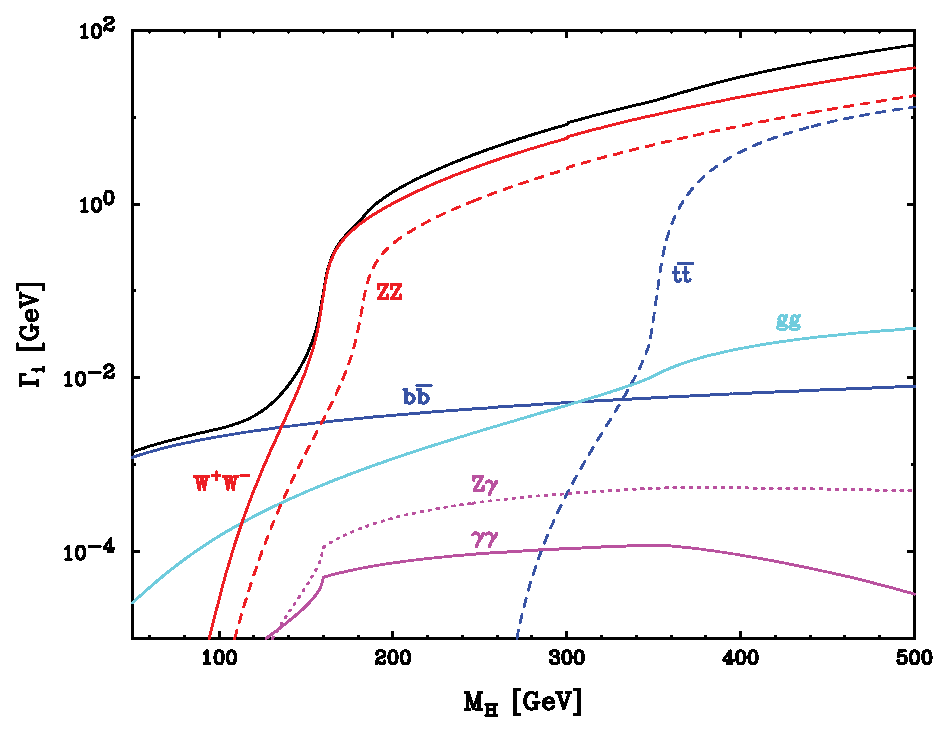
\includegraphics[width=\textwidth]{theory/HiggsDecayWidth}
        \caption{}
        \label{fig:theoryHiggsDecayWidth}
    \end{subfigure}
    \begin{subfigure}[b]{0.45\textwidth}
        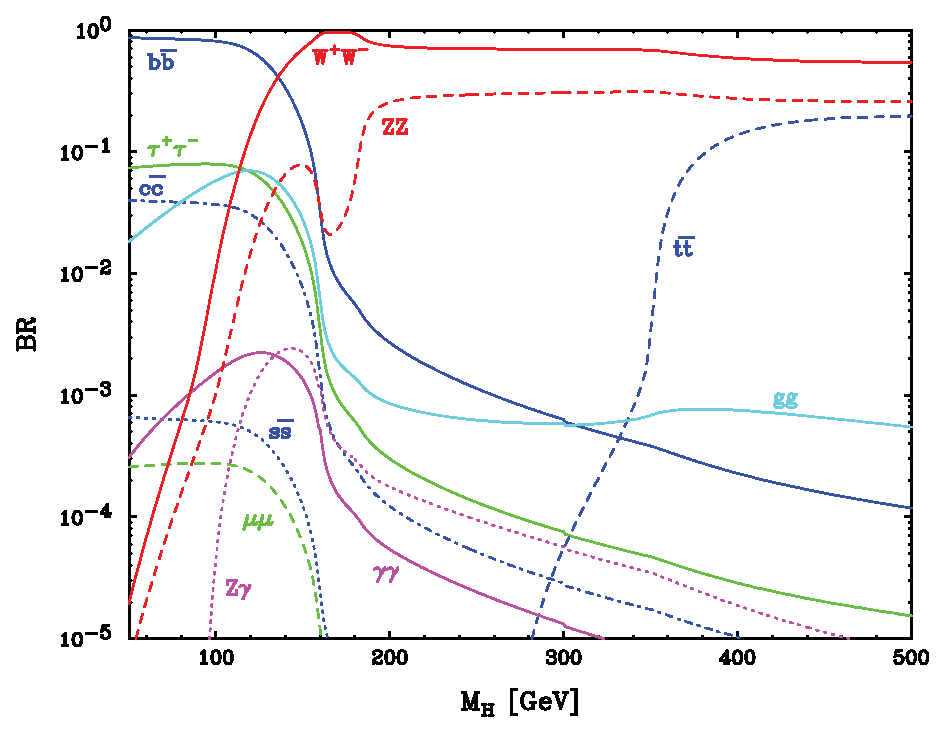
\includegraphics[width=\textwidth]{theory/HiggsBranchingRatio}
        \caption{}
        \label{fig:theoryHiggsBranchingRatio}
    \end{subfigure}
\caption[SM Higgs boson decay width and branching ratios]%
{a) The Higgs boson partial decay widths, and b) Higgs boson branching ratios, plotted as a function of the Higgs boson mass, \Hmass. In a), the black curve shows the total decay width. Both figures are taken from \cite{Rainwater:2007cp}.}
\label{fig:theoryHiggsPhenomenology}
\end{figure}


\section{Yukawa couplings}

The Yukawa sector of the electroweak Lagrangian provides mass terms for quarks and charged leptons after the spontaneous symmetry breaking of the Higgs field. The  corresponding term in the Lagrangian is:
\begin{equation}
\Lagr_{Yukawa} = -\lambda^{u}\overline{q_L}\Phi_{\PH}^{c}u_R  - \lambda^{d}\overline{q_L}\Phi_{\PH}{d}_R - \lambda^{e}\overline{l_L}\Phi_{\PH}e_R + h.c. ,
\end{equation}
where $q_L$ is the left-handed quark doublet field; $u_R$ is the up-type right-handed quark singlet field;  $d_R$ is the down-type right-handed quark singlet field; $l_L$ is the left-handed lepton doublet field; $e_R$ is the right-handed charged lepton singlet field; $\lambda$ is a constant; $\Phi_{\PH}^{c} \equiv i \sigma^2{\PH}^*$ is a SU(2) doublet field with hypercharge $Y = -\frac{1}{2}$; $h.c.$ indicates the Hermitian conjugate terms; and the Lagrangian is summed over all possible quarks and leptons. When the Higgs vacuum expectation value is substituted into $\Lagr_{Yukawa}$, the Yukawa interaction terms give the fermion mass terms:
\begin{equation}
m_{u} = \frac{\lambda^u{\nu}}{\sqrt{2}},\ m_{d} = \frac{\lambda^d{\nu}}{\sqrt{2}},\ m_{e} = \frac{\lambda^e{\nu}}{\sqrt{2}}.
\end{equation}


\section{Beyond the Standard Model Higgs Models}
\label{sec:theoryHiggsBSM}

A number of BSM Higgs theories have been proposed. For example, the light Higgs could be a composite bound state of a new strongly-interacting sector at the TeV scale. If the composite Higgs is  pseudo Nambu-Goldstone boson from spontaneous global symmetry breaking, the Higgs can be naturally light \cite{Kaplan:1983fs}.  In this model, the couplings of the Higgs would deviate from those in the \SM for  Higgs interactions at the TeV scale.


An important physics process for testing the Higgs theory is the double Higgs production via vector boson fusion at the TeV scale \cite{Giudice:2007fh,Contino:2010mh,Contino:2013gna}. For the composite Higgs scenario, the scattering amplitude for this process increases with energy. It is difficult  to measure the double Higgs production at the \LHC due to the large \SM background rate \cite{Contino:2010mh}. However, a multi-TeV electron$-$position linear collider, such as the Compact Linear Collider, would be able to measure the cross section for  this process \cite{Barger:2003rs}.

The study of double Higgs production via \WW fusion can probe the Higgs trilinear self coupling, \gHHH, and quartic coupling, \gWWHH. The coupling \gHHH is associated with the terms in $h^3$ in Higgs potential in \Equation{eq:theoryHiggsSelfCoupling}.   The coupling \gWWHH is associated with the terms in $h^2$ in Higgs interaction terms with other fields in \Equation{eq:theoryHiggsBosonic}. Leading-order Feynman diagrams for double Higgs production via \WW fusion are shown in \Figure{fig:theorydoubleHiggsFeynman}. The diagram shown in  \Figure{fig:theorydoubleHiggsFeynman1} contains the triple Higgs vertex, which is sensitive to the Higgs trilinear self coupling \gHHH. The diagram in \Figure{fig:theorydoubleHiggsFeynman2} is sensitive to the quartic coupling \gWWHH. Figures \ref{fig:theorydoubleHiggsFeynman3} and \ref{fig:theorydoubleHiggsFeynman4} show Feynman diagrams for irreducible background processes containing two \HepProcess{\PH\PWplus\PWminus} vertices.

\begin{figure}[!htbp]
  \begin{subfigure}[b]{0.22\textwidth}
    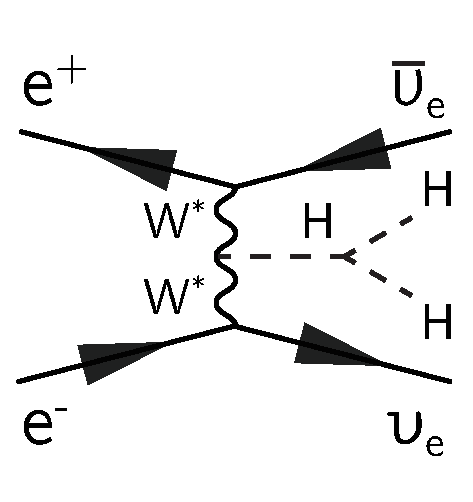
\includegraphics[width=\textwidth]{{{doubleHiggs/Feynman/1}}}
    \caption{}
    \label{fig:theorydoubleHiggsFeynman1}
  \end{subfigure}
  \begin{subfigure}[b]{0.22\textwidth}
    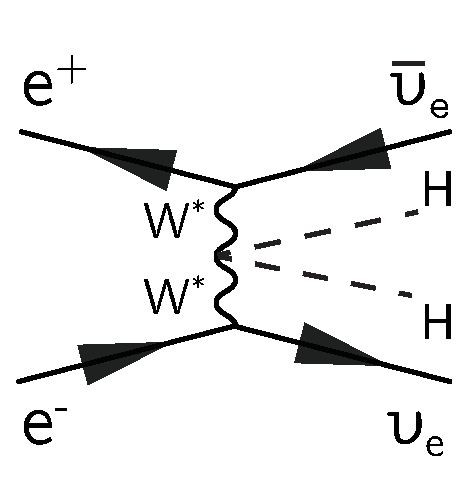
\includegraphics[width=\textwidth]{{{doubleHiggs/Feynman/2}}}
    \caption{}
    \label{fig:theorydoubleHiggsFeynman2}
  \end{subfigure}
  \begin{subfigure}[b]{0.22\textwidth}
    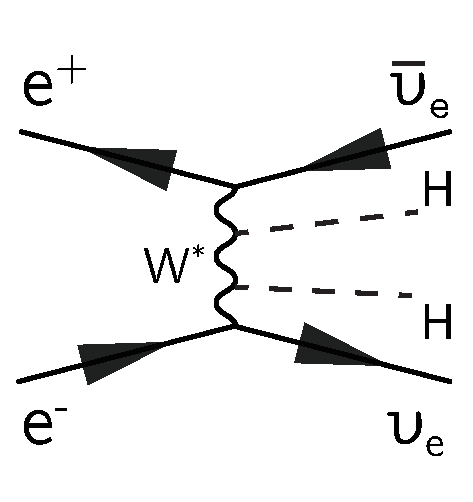
\includegraphics[width=\textwidth]{{{doubleHiggs/Feynman/3}}}
    \caption{}
    \label{fig:theorydoubleHiggsFeynman3}
  \end{subfigure}
  \begin{subfigure}[b]{0.22\textwidth}
    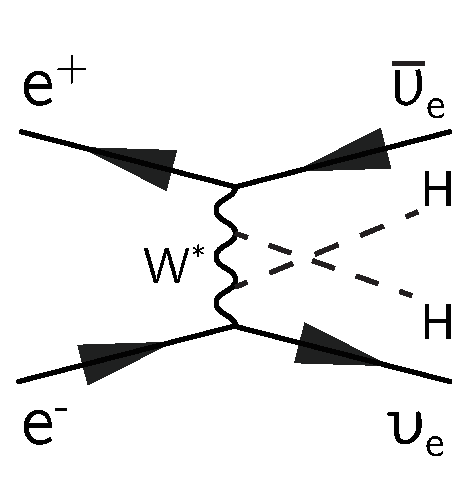
\includegraphics[width=\textwidth]{{{doubleHiggs/Feynman/4}}}
    \caption{}
    \label{fig:theorydoubleHiggsFeynman4}
  \end{subfigure}
\caption
   {The main Feynman diagrams for the leading-order \eeToHH processes.}
   \label{fig:theorydoubleHiggsFeynman}
\end{figure}

Following the assumption made in  \cite{Contino:2010mh,Contino:2013gna}, the self-interaction of the light scalar Higgs, $h$, and its coupling to other \SM bosons can be described by a Lagrangian using the notation in  \cite{Contino:2013gna}. In this description, after the electroweak symmetry breaking , the  Lagrangian is given by:
\begin{equation}
\Lagr =\frac{1}{2}\left(\partial_\mu{h}\right)^2  - V(h) + \parenths{m_W^2{W}_\mu^+{W}^{-\mu} + \frac{m_Z^2}{2}Z_{\mu}Z^\mu}\sqbracs{1 + 2a\frac{h}{\nu} + b \frac{h^2}{\nu^2} + \hdots},
\end{equation}
where $V(h)$ is the $h$ field potential
\begin{equation}
V(h) = \frac{1}{2}m_h^2h^2 + d_3\parenths{\frac{m_h^2}{2\nu}}h^3 + d_4\parenths{\frac{m_h^2}{8{\nu}^2}}h^4 + \hdots ,
\end{equation}
and $a$, $b$, $d_3$ and $d_4$ are  dimensionless parameters. Higher-order terms in $h$ are omitted. The parameters $a$ and $b$ are proportional to the coupling strengths of the $VVh$ and $VVhh$ vertices, where $V$ represents a vector boson, and the parameters $d_3$ and $d_4$ are proportional to the trilinear and quadlinear $h$ self-coupling strength, respectively. Comparing with the  $\Lagr_{Higgs} $ in the \SM (see \Equation{eq:theoryHiggsBosonic} and \Equation{eq:theoryHiggsSelfCoupling}),  it can be seen that $a=b=d_3=d_4=1$ in the \SM, and all higher order terms vanish. However, BSM Higgs model allow $a,b,d_3,d_4$ to take different values.

Consider a pair of the longitudinal polarised  vector bosons (${V}_L$) coupling to two $h$ fields. The scattering amplitude for \HepProcess{{V}_L{V}_L \to hh} can be written as:
\begin{equation}
A = a^2\parenths{A_{SM} + A_1\delta_b + A_2\delta_{d_3}},
\end{equation}
where $A_{SM}$ is the \SM amplitude and:
\begin{equation}
\delta_b  & \equiv 1 - \frac{b}{a^2}, \\
\delta_{d_3} & \equiv 1 - \frac{d_3}{a}.
\end{equation}
The term $A_1$ grows like the square of energy at a large center-of-mass energy, $E\gg{m_V}$. The terms $A_{SM}$ and $A_2$ have no energy dependence. Therefore, the parameter $\delta_b$ controls the magnitude of the increasing of the scattering amplitude as a function of energy.  In an electron$-$positron collider, this scattering process can be studied via the double Higgs production \HepProcess{\Ppositron\Pelectron \to \Pneutrino\APneutrino hh} channel, where the cross section can be written as
\begin{equation}
\label{eq:theoryGeneralHiggsCrossSection}
\sigma = a^4\sigma_{SM}\parenths{1 + A\delta_b + B\delta_{d_3} + C\delta_b\delta_{d_3} + D\delta_b^2 + E\delta_{d_3}^2},
\end{equation}
% The parameter $\delta_{d_3}$, on the other hand, determines the magnitude at the higgs mass threshold.
where $\sigma_{SM}$ is the \SM cross section. Variables that increase with the increasing of the centre-of-mass energies are suitable for studying the cross section dependence on parameters $\delta_{b}$ and $\delta_{d_3}$. Two examples of such variables are the invariant mass of the two Higgs system, $m_{hh}$, and the scalar sum of two Higgs transverse momenta, $H_T$. \FIGURE{fig:theoryMhhHtDistribution} shows that the $m_{hh}$ and $H_T$ distributions are sensitive to the values of $\delta_{b}$ and $\delta_{d_3}$  \cite{Contino:2013gna}.  The changes in the  $m_{hh}$ and $H_T$ distributions can be related to the  change in $\delta_{b}$ and $\delta_{d_3}$. Therefore deviations of  $\delta_{b}$ and $\delta_{d_3}$ from those \SM values, 1, could be established using the $m_{hh}$ and $H_T$ distributions. It should be noted that  \Figure{fig:theoryMhhHtDistribution} shows a generator-level study; detector effect will affect the distributions because of, for example, the loss of the reconstruction efficiency in the  barrel/endcap overlap region.

%a study of sensitivity of the $\delta_{b}$ and $\delta_{d_3}$ can be established using the $m_{hh}$ and $H_T$ distributions. It should be noted that the \Figure{fig:theoryMhhHtDistribution} is obtained from a generator-level study.
%Around the \SM value of $\delta_{d_3}$, a large value of $\delta_{b} $(0.3) produces events with large values of $m_{hh}$ and $H_T$.
\begin{figure}[htbp]
\centering
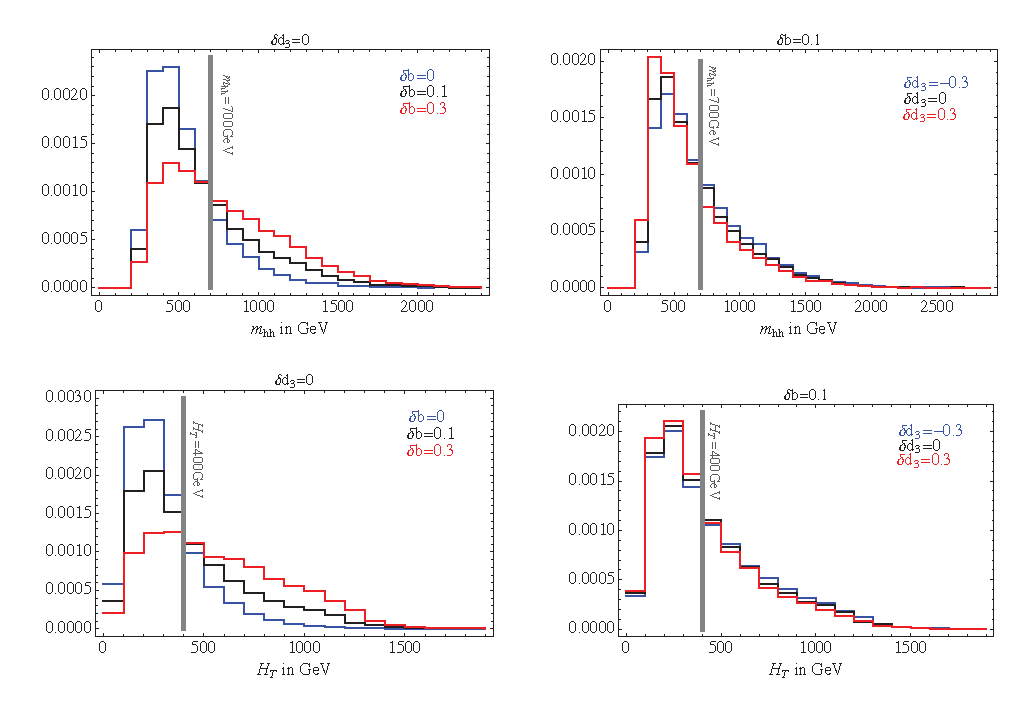
\includegraphics[width=1\textwidth]{theory/MhhHtDistribution}
\caption[]
{Normalised differential cross sections $d\sigma/dm_{hh}$ and $d\sigma/dH_{T}$ for \HepProcess{\Ppositron\Pelectron \to \Pneutrino\APneutrino hh} for \CLIC at \rootS{3} after applying generator-level identification cuts,  for several values of $\delta_{b}$ and $\delta_{d_3}$. The plot is taken from \cite{Contino:2013gna}.}
\label{fig:theoryMhhHtDistribution}
\end{figure}

In the expression of the cross section of the double Higgs production via \HepProcess{\Ppositron\Pelectron \to \Pneutrino\APneutrino hh}  in \Equation{eq:theoryGeneralHiggsCrossSection}, the parameter $a$, which is proportional to $g_{VVH}$, enters as an overall factor. \FIGURE{fig:theoryHiggsCrossSection} shows the comparison of cross sections as a function of the centre-of-mass energy, for different the Higgs production modes. Up to a centre-of-mass energy of \rootS{3}, the cross sections of the single Higgs production are two orders of magnitude larger than the cross sections of the double higgs production. The cross section of  \HepProcess{\Ppositron\Pelectron \to \Pneutrino\APneutrino h} channel is given by:
\begin{equation}
\sigma = \sigma_{SM}\parenths{1 + A\Delta{a} + B\Delta{a}^2},
\end{equation}
where $\Delta{a}\equiv 1 - a$ is the change in $a$, and $A$ and $B$ are two dimensionless coefficients.  The measurement of the parameter $a$, using  \HepProcess{\Ppositron\Pelectron \to \Pneutrino\APneutrino h}  channel, would be performed before the measurement of the $\delta_{b}$ and $\delta_{d_3}$ for the double Higgs production.

\begin{figure}[!htbp]
\centering
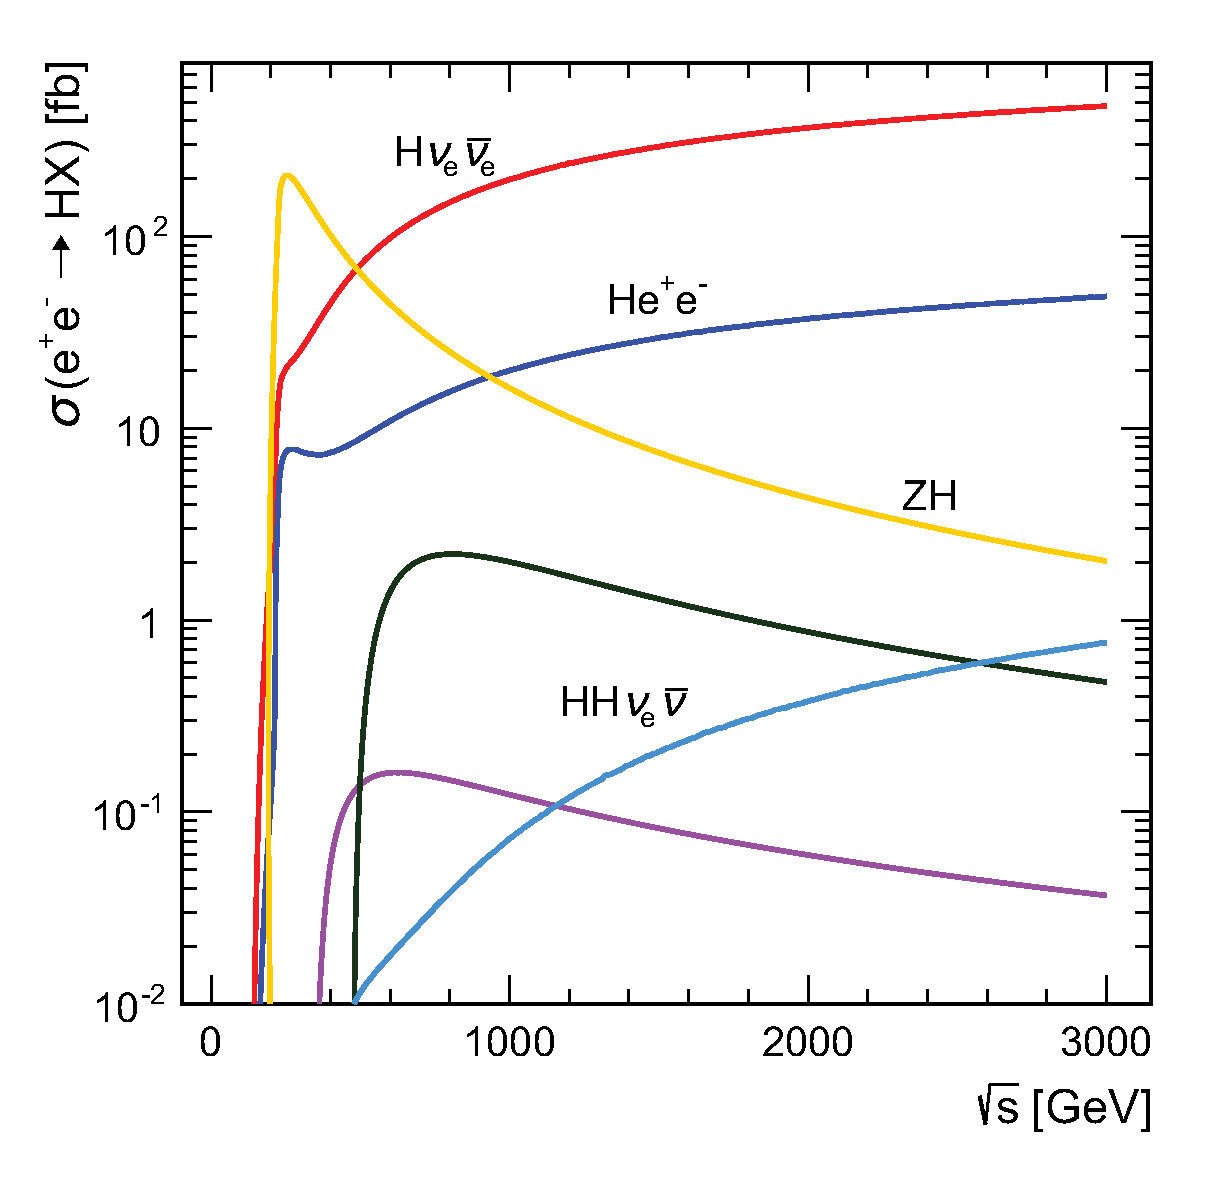
\includegraphics[width=0.45\textwidth]{theory/HiggsCLICcrossSection}
\caption[]
{Cross sections as a function of centre-of-mass energy for Higgs production processes at an electron-positron collider for a Higgs mass of 126\,GeV. The cross section values correspond to unpolarised beams and do not include the effect of beamstrahlung. The plot is taken from \cite{Abramowicz:2016zbo}.}
\label{fig:theoryHiggsCrossSection}
\end{figure}


Therefore, for the purpose of measuring $g_{VVHH}$ and $g_{HHH}$ via double Higgs production, it is sufficient to treat the parameter $a$ as a known constant. Hence only a two-dimensional fit of the parameters $\delta_{b}$ and $\delta_{d_3}$ would be performed to extract values of $\delta_{b}$ and $\delta_{d_3}$.

%However,  for a multi-TeV electron-positron collider, the cross section for single Higgs production is far greater than that of the double Higgs production.

%Therefore, for the purpose of measuring $g_{VVHH}$ and $g_{HHH}$ via double Higgs production, it is sufficient to treat the parameter $a$ as a known constant. Hence only a two-dimensional fit of the parameters $\delta_{b}$, and $\delta_{d_3}$ would be performed.



%In the cross section of the double Higgs production via \HepProcess{\Ppositron\Pelectron \to \Pneutrino\APneutrino hh}  in \Equation{eq:theoryGeneralHiggsCrossSection}, the parameter $a$, which is proportional to $g_{VVH}$, enters as an overall factor. At the same time, $a$ also appears in the definition of $\delta_{b}$ and $\delta_{d_3}$. Hence a three-dimensional fit of the parameters $a$, $\delta_{b}$, and $\delta_{d_3}$ would be needed to extract the values of the$a$, $\delta_{b}$, and $\delta_{d_3}$. However,  for a multi-TeV electron-positron collider, the cross section for single Higgs production is far greater than that of the double Higgs production. Consequently, the measurement of the parameter $a$, using  \HepProcess{\Ppositron\Pelectron \to \Pneutrino\APneutrino h}  channel, would be performed before the measurement of the $\delta_{b}$ and $\delta_{d_3}$ for the double Higgs production.

\section{Tau pair polarisation correlations as a signature of Higgs boson}
\label{sec:theoryTauPair}


The tau lepton has been studied extensively in the past at the Large Electron$-$Positron Collider (LEP)\cite{Schael:2005am}.  The tau lepton is a fundamental particle, with a negative electric charge and a spin of $\frac{1}{2}$. It has the same fundamental interaction property as an electron, but a much larger mass. Unlike the stable electron, because the tau lepton is massive, it decays via the weak interaction with a mean decay lifetime of $(290.3\pm0.5)\times10^{-15}$\,s \cite{Abreu:1991jn}. The tau lepton has many decay modes. The decay modes with branching ratio above 2\% are listed in \Table{tab:theoryTauDecayMode}.

% The most difficult final states to separate are \decayRhoFinalStateShort and \decayAiPhotonFinalStateShort, where photons from boosted \Ppizero are very challenging to reconstruct correctly.

\begin{table}[htbp]\centering
\smallskip
\begin{tabular}{l l r}
\hline
\hline
Decay modes & Final states & Branching ratio\\
\hline
\decayElectron   &  \decayElectron  & $17.83{\pm0.04\%}$   \\
\decayMuon &	\decayMuon & $17.41{\pm0.04\%}$  \\
\decayPion  &   \decayPion	& $10.83{\pm0.06\%}$   \\
\decayRho   & \decayRhoFinalState& $25.52{\pm0.09\%}$ \\
\decayAi   neutral& \decayAiPhotonFinalState	& $9.30{\pm0.11\%}$    \\
\decayAi  charged&	\decayAiPionFinalState    & $8.99{\pm0.06\%}$  \\
\decayThreePionPhoton  &	\decayThreePionPhoton    & $2.70{\pm0.08\%}$  \\
\hline
\hline
\end{tabular}
\caption[Decay modes, final state particles and branching ratios of the seven major \Pgtm decays.]
{Decay modes, final state particles, and branching ratios of the seven major \Pgtm decays, taken from \cite{Agashe:2014kda}.}
\label{tab:theoryTauDecayMode}
\end{table}

A scalar Higgs boson with spin-0 can decay to \TauTauSub{L}{L} or \TauTauSub{R}{R}, whereas  a vector boson \PZ with spin-1 can decay to \TauTauSub{L}{R} or \TauTauSub{R}{L}, where L, R denotes the tau lepton helicity. Therefore, by studying the correlation between the polarisations of the  tau pair from a boson decay, one can determine statistically if the parent boson is a  scalar or a vector.

%For many theories beyond the Standard Model, a common feature is that the coupling of the Higgs particle to leptons increases with the increase of the lepton mass \cite{Duperrin:2008in}.  In these BSM theories, unlike vector bosons coupling to all flavours of leptons equally, the \HigssTauTau coupling would dominate the Higgs coupling to leptons. Therefore, if an experiment observes the breaking of the lepton universality by favouring \TauTau events, it could indicate the existence of a scalar Higgs. When such a universality breaking is observed, a helicity correlation test can be used to show that the \TauTau pair is from a scalar boson or a vector boson. In particular, the polarisation correlations of tau leptons are different for \HiggsToTauTau and \ZToTauTau, as scalar Higgs decays to \TauTauSub{L}{L} or \TauTauSub{R}{R} and \PZ decays to \TauTauSub{L}{R} or \TauTauSub{R}{L}, where L, R denotes the tau lepton helicities.


The tau pair polarisation correlation can be studied using various tay decay modes. Here \Reference{Bullock:1991my} is followed and the \tauToPionBoth decay mode is used as the example. The Higgs and \PZ boson decay to a  tau pair, where both tau leptons subsequently decay   via  \tauToPionBoth, can be represented as:
\begin{equation}
\HepProcess{X \to \TauTauSub{\alpha}{\beta} \to \Ppiplus\Ppiminus  + \Pneutrino{s}},
\end{equation}
where $X$ is either \PHiggs or \PZ, and $\alpha$, $\beta$ are the tau lepton helicities, L or R. In the collinear limit where $m^2_{\Ptau}/m^2_X \ \ll \ 1$, the appropriate kinematic variables are the energy fractions:
\begin{equation}
z & = \frac{E_{\Ppiminus}}{E_{\Ptauon}}, \\
\overline{z} & = \frac{E_{\Ppiplus}}{E_{\APtauon}}.
\end{equation}

For a single tau decay, the differential cross section distribution can be written as:
\begin{equation}
\frac{1}{\Gamma_{\Ptau}}\frac{d\Gamma}{dz} = Br{\parenths{\tauToPion}} f\parenths{\HepProcess{\TauFull{\alpha}{-} \to \Ppiminus} ; z},
\end{equation}
where $Br{\parenths{\tauToPion}}$ is the branching fraction of \tauToPion decay mode. The form $f$ can be obtained by working out the matrix element from the Feynman diagram and integrating  the square of the matrix element over the phase space \cite{Tsai:1971vv}:
\begin{equation}
f\parenths{\HepProcess{\TauFull{\alpha}{-} \to \Ppiminus} ; z} = 1 + P_\alpha\parenths{2z-1},
\end{equation}
where $P_L = -1$ and $P_R = +1$. Hence for the tau pair decay, the differential cross section distribution is of the form:
\begin{equation}
\frac{d^2N\parenths{\HepProcess{X \to \TauTau \to \Ppiplus\Ppiminus  + \Pneutrino's}}}{dz\,d\overline{z}} = \parenths{Br{\parenths{\tauToPion}}}^2 \sum_{\alpha,\,\beta}^{} C^X_{\alpha \beta} f\parenths{\HepProcess{\TauFull{\alpha}{-} \to \Ppiminus} ; z} f\parenths{\HepProcess{\TauFull{\beta}{+} \to \Ppiplus} ; \overline{z}},
\end{equation}
where the only non-zero correlation coefficients $C_{\alpha \beta}$ for the parity-conserving \HiggsToTauTau are:
\begin{equation}
C^{\PHiggs}_{LL} = C^{\PHiggs}_{RR} = \frac{1}{2}.
\end{equation}
In contrast, the non-zero correlation coefficients  for the  \ZToTauTau are:
\begin{equation}
C^{\PZ}_{LR} = \frac{1}{2}\parenths{1 - P_{\Ptau}},\ C^{\PZ}_{RL} = \frac{1}{2}\parenths{1 + P_{\Ptau}},
\end{equation}
where $P_{\Ptau}$ is the mean  non-zero tau polarisation of \PZ decays. The tau polarisation is not zero because the process \ZToTauTau  is not parity-conserving. In the \SM:
\begin{equation}
P_{\Ptau} = \frac{-2va}{v^2 + a^2},
\end{equation}
where the parameter $v= -\frac{1}{2} + \sin^2{\theta_{\PW}}$ and  $a= -\frac{1}{2}$ are the respective vector and axial-vector \ZTauTau couplings.


\FIGURE{fig:theoryTauPairCorrelation} shows the resulting two-dimensional distributions of  $\overline{z} = \frac{E_{\Ppiplus}}{E_{\APtauon}}$ versus  $z = \frac{E_{\Ppiminus}}{E_{\Ptauon}}$ for \ZToTauTau and \HiggsToTauTau channels, where both tau leptons decay via \tauToPionBoth. The difference of the tau pair polarisation correlation between \PZ and \PHiggs  is clear. The energy distribution of the charged pion from \ZToTauTau has the form of $\overline{z}  \sim z$, whilst the distribution from  \HiggsToTauTau has the form of $\overline{z}  \sim (1-z)$. Therefore, in \ZToTauTau process, a high-energy \Pgppm  is likely to be associated with a high-energy \Pgpmp. In \HiggsToTauTau process, the opposite is favoured. If the tau pair decay from Higgs boson is observed, the decay can be recognised in the \tauToPionBoth mode as a high-energy \Pgppm with a low-energy \Pgpmp. Hence, the tau decay product energy distribution can be used as a signature for \HiggsToTauTau.

%Photon - passage through matter. Photon electromagnetic shower

\begin{figure}[htbp]
\centering % \begin{center}/\end{center} takes some additional vertical space
%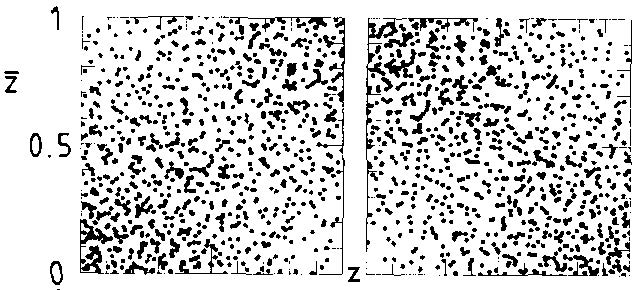
\includegraphics[width=0.9\textwidth]{theory/TauPairCorrelation.jpg}
  \begin{subfigure}[t]{0.45\textwidth}
    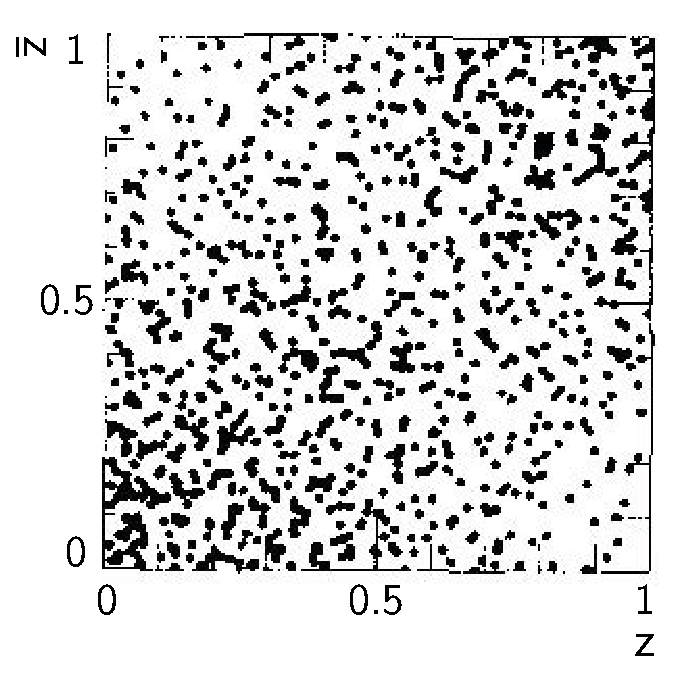
\includegraphics[width=\textwidth]{theory/TauZ}
    \caption{\ZToTauTau}
    \label{fig:theoryTauPairCorrelationZ}
  \end{subfigure}
  \begin{subfigure}[t]{0.45\textwidth}
    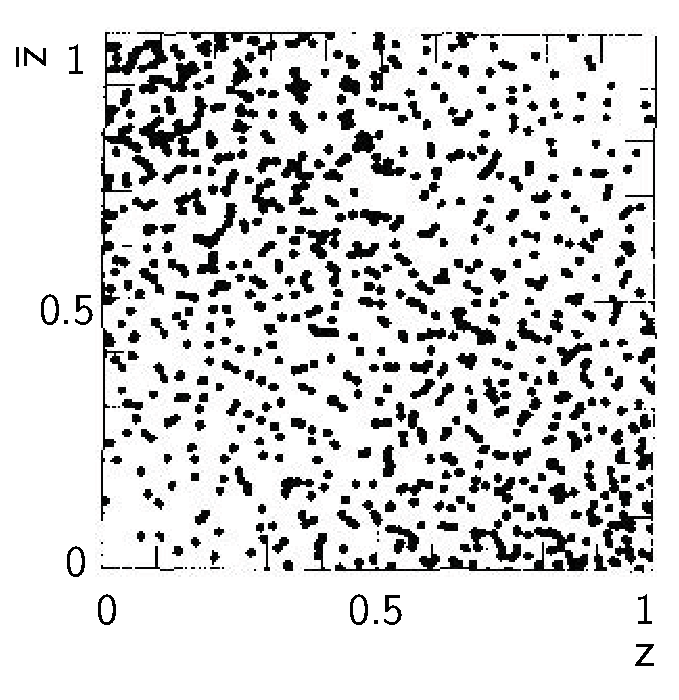
\includegraphics[width=\textwidth]{theory/TauH}
    \caption{\HiggsToTauTau}
    \label{fig:theoryTauPairCorrelationH}
  \end{subfigure}
\caption[Two-dimensional distribution of \ZToTauTau and \HiggsToTauTau.]
{Two-dimensional distribution of $\overline{z} ={E_{\Ppiplus}}/{E_{\APtauon}}$ plotted against $ z ={E_{\Ppiminus}}/{E_{\Ptauon}}$  for a) \ZToTauTau, and b) \HiggsToTauTau processes, where both tau leptons decay via \tauToPionBoth, adapted from reference \cite{Tsai:1971vv}.}
\label{fig:theoryTauPairCorrelation}
\end{figure} 